% ============================================================
%  يُترجَم بـ XeLaTeX  (في Overleaf: Menu → Compiler → XeLaTeX)
%  الخط: Amiri (متوفر في Overleaf، أو حمّله من github.com/aliftype/amiri)
% ============================================================
\documentclass[12pt,a4paper]{article}
\usepackage[a4paper,margin=1.7cm,top=2.3cm,bottom=2.9cm,headheight=15pt,footskip=1.5cm]{geometry}
\usepackage{amsmath,amssymb}
\usepackage{icomma}
\usepackage[english,bidi=default,layout=lists]{babel}
\babelprovide[import,main]{arabic}
\babelfont{rm}[Scale=1.08]{Amiri}
\babelfont{sf}[Scale=1.08]{Amiri}
\usepackage[most]{tcolorbox}
\usepackage{tikz}
\usetikzlibrary{arrows.meta,calc,shadings}
\usepackage{array}
\usepackage{colortbl}
\usepackage{fancyhdr}
\usepackage{titlesec}
\usepackage{enumitem}
\usepackage{collcell}
\usepackage{needspace}
\usepackage{etoolbox}
% أعمدة جداول تُكتب خلاياها بالعربية في الاتجاه الصحيح
\newcolumntype{C}{>{\collectcell\ar}c<{\endcollectcell}}
% تجنب عنوان يتيم في أسفل الصفحة
\pretocmd{\section}{\Needspace{15\baselineskip}}{}{}
\pretocmd{\subsection}{\Needspace{11\baselineskip}}{}{}

% ---------- الألوان ----------
\definecolor{cDef}{HTML}{1F4E9C}
\definecolor{cThm}{HTML}{B3261E}
\definecolor{cRem}{HTML}{2E7D32}
\definecolor{cEx}{HTML}{C76B00}
\definecolor{cMeth}{HTML}{6A1B9A}
\definecolor{cSol}{HTML}{00695C}
\definecolor{cSec}{HTML}{1F3A68}

% ---------- العناوين ----------
\titleformat{\section}{\Large\bfseries\color{cSec}}{\thesection.}{0.6em}{}[{\color{cSec!60}\titlerule[1pt]}]
\titleformat{\subsection}{\large\bfseries\color{cThm!85!black}}{\thesubsection.}{0.5em}{}
\titlespacing*{\section}{0pt}{14pt}{8pt}
\titlespacing*{\subsection}{0pt}{10pt}{5pt}
\setlength{\parindent}{0pt}
\setlength{\parskip}{4pt}
\setlist{itemsep=2pt,topsep=3pt}

% ---------- الصناديق (تُرسم في سياق LTR ويُكتب محتواها بالعربية) ----------
\newtcolorbox{arbox}[3][]{enhanced,
  colback=#2!5,colframe=#2!80!black,arc=2mm,boxrule=0.8pt,
  left=6pt,right=6pt,top=8pt,bottom=5pt,
  fonttitle=\bfseries,coltitle=white,
  title={\foreignlanguage{arabic}{#3}},
  attach boxed title to top right={xshift=-5mm,yshift=-3mm},
  boxed title style={colback=#2!80!black,arc=1.5mm,boxrule=0pt},
  before upper={\selectlanguage{arabic}},
  before skip=8pt,after skip=8pt,breakable,#1}
\newenvironment{BOX}[2]{\begin{otherlanguage}{english}\begin{arbox}{#1}{#2}}{\end{arbox}\end{otherlanguage}}
\newenvironment{tarif}[1][تعريف]{\begin{BOX}{cDef}{#1}}{\end{BOX}}
\newenvironment{khassia}[1][خاصية]{\begin{BOX}{cThm}{#1}}{\end{BOX}}
\newenvironment{molahada}[1][ملاحظة]{\begin{BOX}{cRem}{#1}}{\end{BOX}}
\newenvironment{mithal}[1][مثال]{\begin{BOX}{cEx}{#1}}{\end{BOX}}
\newenvironment{tariqa}[1][طريقة]{\begin{BOX}{cMeth}{#1}}{\end{BOX}}

% ---------- التمارين والحلول ----------
\newcounter{exo}
\newenvironment{tamrin}[1]{\stepcounter{exo}\begin{BOX}{cSec}{التمرين \theexo: #1}}{\end{BOX}}
\newenvironment{hal}{\Needspace{12\baselineskip}\begin{otherlanguage}{english}\begin{arbox}[breakable]{cSol}{حل التمرين \theexo}}{\end{arbox}\end{otherlanguage}}

% رسومات TikZ تُوضع في سياق LTR
\newenvironment{LTR}{\begin{otherlanguage}{english}}{\end{otherlanguage}}
\newcommand{\ar}[1]{\foreignlanguage{arabic}{#1}}

% ---------- رموز ----------
% نقاط الحذف داخل الرياضيات (\dots يسبب خللاً في الاتجاه مع babel)
\renewcommand{\dots}{\mathinner{\ldotp\ldotp\ldotp}}
\renewcommand{\ldots}{\mathinner{\ldotp\ldotp\ldotp}}
\renewcommand{\cdots}{\mathinner{\cdotp\cdotp\cdotp}}
\newcommand{\N}{\mathbb{N}}
\newcommand{\Z}{\mathbb{Z}}
\newcommand{\D}{\mathbb{D}}
\newcommand{\Q}{\mathbb{Q}}
\newcommand{\R}{\mathbb{R}}
\newcommand{\pgcd}{\operatorname{PGCD}}
\newcommand{\ppcm}{\operatorname{PPCM}}

% ---------- تمثيل مجال على مستقيم عددي ----------
% \NLseg{a}{b}{[}{]}  مجال محدود
\newcommand{\NLseg}[4]{\begin{LTR}\begin{tikzpicture}[baseline=-0.6ex]
 \draw[-{Stealth[length=2mm]},gray!70](0,0)--(3.4,0);
 \draw[line width=2pt,cThm!80!black](0.7,0)--(2.7,0);
 \node[cThm!80!black,font=\LARGE] at (0.7,0){$#3$};
 \node[cThm!80!black,font=\LARGE] at (2.7,0){$#4$};
 \node[below=3pt,font=\footnotesize] at (0.7,0){$#1$};
 \node[below=3pt,font=\footnotesize] at (2.7,0){$#2$};
\end{tikzpicture}\end{LTR}}
% \NLright{a}{[}  مجال نحو +∞
\newcommand{\NLright}[2]{\begin{LTR}\begin{tikzpicture}[baseline=-0.6ex]
 \draw[-{Stealth[length=2mm]},gray!70](0,0)--(3.4,0);
 \draw[line width=2pt,cThm!80!black](1.3,0)--(3.3,0);
 \node[cThm!80!black,font=\LARGE] at (1.3,0){$#2$};
 \node[below=3pt,font=\footnotesize] at (1.3,0){$#1$};
\end{tikzpicture}\end{LTR}}
% \NLleft{b}{]}  مجال نحو −∞
\newcommand{\NLleft}[2]{\begin{LTR}\begin{tikzpicture}[baseline=-0.6ex]
 \draw[-{Stealth[length=2mm]},gray!70](0,0)--(3.4,0);
 \draw[line width=2pt,cThm!80!black](0.05,0)--(2.1,0);
 \node[cThm!80!black,font=\LARGE] at (2.1,0){$#2$};
 \node[below=3pt,font=\footnotesize] at (2.1,0){$#1$};
\end{tikzpicture}\end{LTR}}

% ---------- أيقونات مواقع التواصل (مرسومة بـ TikZ، لا تحتاج أي حزمة) ----------
\definecolor{cFB}{HTML}{1877F2}
\definecolor{cTG}{HTML}{229ED9}
\definecolor{cIG1}{HTML}{FEDA75}
\definecolor{cIG2}{HTML}{D62976}
\definecolor{cIG3}{HTML}{4F5BD5}
\newcommand{\fbicon}{\begin{LTR}\begin{tikzpicture}[baseline=-0.75ex,x=1em,y=1em]
 \fill[cFB] (0,0) circle (0.55);
 \node[white,inner sep=0,font=\usefont{TU}{lmss}{bx}{n}\small] at (0.04,-0.02) {f};
\end{tikzpicture}\end{LTR}}
\newcommand{\igicon}{\begin{LTR}
\begin{tikzpicture}[baseline=-0.75ex,x=1em,y=1em]
 \shade[lower left=cIG1,lower right=cIG2,upper left=cIG2,upper right=cIG3,rounded corners=0.28em] (-0.55,-0.55) rectangle (0.55,0.55);
 \draw[white,line width=0.09em,rounded corners=0.18em] (-0.36,-0.36) rectangle (0.36,0.36);
 \draw[white,line width=0.09em] (0,0) circle (0.17);
 \fill[white] (0.22,0.22) circle (0.05);
\end{tikzpicture}\end{LTR}}
\newcommand{\tgicon}{\begin{LTR}
\begin{tikzpicture}[baseline=-0.75ex,x=1em,y=1em]
 \fill[cTG] (0,0) circle (0.55);
 \fill[white] (-0.33,0.0) -- (0.32,0.27) -- (0.2,-0.3) -- (0.0,-0.15) -- (-0.08,-0.28) -- (-0.08,-0.08) -- cycle;
 \fill[cTG!70!black] (-0.08,-0.08) -- (0.25,0.2) -- (0.0,-0.15) -- (-0.08,-0.28) -- cycle;
\end{tikzpicture}\end{LTR}}
% سطر مواقع التواصل أسفل كل صفحة
% (يُكتب السطر بترتيب بصري من اليسار إلى اليمين: الأيقونة يمين كل اسم)
\newcommand{\PageBox}{\begin{LTR}\tikz[baseline=(p.base)]\node[fill=black,text=white,inner sep=2.5pt,minimum width=1.6em,minimum height=1.3em,font=\usefont{TU}{lmss}{bx}{n}\small](p){\ifnum\value{page}<10 0\fi\arabic{page}};\end{LTR}}
\newcommand{\SocialRow}{\begin{otherlanguage}{english}%
 \ar{\textbf{الأستاذ سوايسية هشام للرياضيات}}\ \tgicon\hfill
 \textbf{prof\_hicham\_math}\ \igicon\hfill
 \ar{\textbf{الأستاذ سوايسية هشام للرياضيات}}\ \fbicon\hspace{2.2em}\PageBox\end{otherlanguage}}
% ---------- رأس وتذييل الصفحة ----------
\pagestyle{fancy}
\fancyhf{}
\renewcommand{\headrulewidth}{0.6pt}
\renewcommand{\footrulewidth}{0.4pt}
% \SetHeader{يمين الرأس}{يسار الرأس}{يمين التذييل}{يسار التذييل}
\newcommand{\SetHeader}[2]{%
 \fancyhead[C]{\parbox{\textwidth}{\ar{#1\hfill #2}}}%
 \fancyfoot[C]{\parbox{\textwidth}{\small\SocialRow}}}

\usepackage{tkz-tab}
\usepackage{multicol}
% جدول تغيرات / إشارة (يُرسم في سياق LTR)
\newenvironment{TAB}{\par\begin{center}\begin{LTR}\begin{tikzpicture}[scale=0.95,every node/.style={font=\small}]}{\end{tikzpicture}\end{LTR}\end{center}}
% معلم بشبكة: \begin{GR}{xmin}{xmax}{ymin}{ymax}{unit cm}
\newenvironment{GR}[5]{\par\begin{center}\begin{LTR}\begin{tikzpicture}[x=#5cm,y=#5cm,font=\footnotesize]
 \def\xmn{#1}\def\xmx{#2}\def\ymn{#3}\def\ymx{#4}
 \draw[gray!25,very thin] (#1,#3) grid (#2,#4);
 \draw[-{Stealth[length=2mm]}] (#1,0)--(#2+0.3,0) node[below left]{$x$};
 \draw[-{Stealth[length=2mm]}] (0,#3)--(0,#4+0.3) node[below left]{$y$};
 \node[below left] at (0,0){$O$};
 \draw[very thick,-{Stealth[length=1.6mm]}] (0,0)--(1,0) node[below,pos=.55]{$\vec i$};
 \draw[very thick,-{Stealth[length=1.6mm]}] (0,0)--(0,1) node[left,pos=.55]{$\vec j$};
 \begin{scope}\clip (#1,#3) rectangle (#2,#4);}
{\end{scope}\end{tikzpicture}\end{LTR}\end{center}}
\newcommand{\Ticks}[2]{\foreach \t in {#1} \node[below,font=\scriptsize] at (\t,0){$\t$}; \foreach \t in {#2} \node[left,font=\scriptsize] at (0,\t){$\t$};}
\newcommand{\bx}[1]{\ensuremath{\colorbox{cDef!12}{$\displaystyle #1$}}}
\newcommand{\hl}[1]{\ensuremath{\colorbox{cEx!20}{$\displaystyle #1$}}}
\newcommand{\Lim}[1]{\displaystyle\lim_{x\to #1}}
\newcommand{\Cf}{(C_f)}
\newenvironment{qst}{\begin{enumerate}[label=\protect\circled{\arabic*},leftmargin=*]}{\end{enumerate}}
\newcommand{\circled}[1]{\foreignlanguage{english}{\tikz[baseline=(c.base)]\node[circle,fill=cDef,text=white,inner sep=1.2pt,font=\scriptsize\bfseries](c){#1};}}
% عمودان: \TwoCol{عرض اليسار}{محتوى اليسار}{عرض اليمين}{محتوى اليمين}  (آمن مع TikZ)
\newcommand{\TwoCol}[4]{\par\begin{LTR}\noindent\begin{minipage}[t]{#1\textwidth}\selectlanguage{arabic}#2\end{minipage}\hfill\begin{minipage}[t]{#3\textwidth}\selectlanguage{arabic}#4\end{minipage}\end{LTR}\par}
\newcommand{\un}{(u_n)}\newcommand{\vn}{(v_n)}
% برهان بالتراجع: \Rec{الخاصية P(n)}{التحقق من P(0)}{البرهان على الوراثة}
\newcommand{\Rec}[3]{\textbf{برهان بالتراجع:} نسمي $P(n)$ الخاصية: «#1».
\begin{itemize}
\item \textbf{التحقق:} #2
\item \textbf{الوراثة:} نفرض أن $P(n)$ صحيحة ونبرهن صحة $P(n+1)$: #3
\item \textbf{الخلاصة:} حسب مبدأ الاستدلال بالتراجع، $P(n)$ صحيحة من أجل كل عدد طبيعي $n$.
\end{itemize}}
\newcommand{\src}[1]{{\footnotesize\textbf{#1}}\par}
\newcommand{\ok}{$\textcolor{cRem}{\checkmark}$}
\newcommand{\limn}{\displaystyle\lim_{n\to+\infty}}
% أسئلة فرعية (أ) (ب) (جـ) كل سؤال في سطر
\newenvironment{sq}{\begin{itemize}[leftmargin=2.4em,itemsep=3pt]}{\end{itemize}}
\newcommand{\qa}{\item[(أ)]}\newcommand{\qb}{\item[(ب)]}\newcommand{\qc}{\item[(جـ)]}\newcommand{\qd}{\item[(د)]}\newcommand{\qe}{\item[(هـ)]}
\newcommand{\pa}{\par\smallskip\textbf{(أ)} }\newcommand{\pb}{\par\smallskip\textbf{(ب)} }\newcommand{\pc}{\par\smallskip\textbf{(جـ)} }\newcommand{\pd}{\par\smallskip\textbf{(د)} }\newcommand{\pe}{\par\smallskip\textbf{(هـ)} }
\newcommand{\ccl}[1]{\par\textbf{الخلاصة:} #1}

\SetHeader{\small\bfseries\color{cSec}ملخص: المتتاليات العددية}{\small\color{cSec}السنة الثانية ثانوي -- الشعب العلمية}
\begin{document}
\newcolumntype{M}[1]{>{\centering\arraybackslash}p{#1}}
\newcommand{\RL}[4]{\TwoCol{#3}{#4}{#1}{#2}}
\newcommand{\QQ}[1]{\par\smallskip\textbf{#1.} }
\newenvironment{tmr}{\stepcounter{exo}\begin{BOX}{cSec}{تمرين محلول \theexo}}{\end{BOX}}
\newcommand{\Un}{(u_n)}
\begin{LTR}
\begin{tcolorbox}[enhanced,colback=cSec,colframe=cSec,arc=3mm,halign=center,boxrule=0pt,top=12pt,bottom=12pt,before upper={\selectlanguage{arabic}}]
{\color{white}\fontsize{28}{34}\selectfont\bfseries المتتاليات العددية}\\[8pt]
{\color{white}\large ملخص شامل مع أمثلة وأشكال وتمارين محلولة خطوة بخطوة}\\[5pt]
{\color{white}\large السنة الثانية ثانوي -- الشعب العلمية (رياضيات ، تقني رياضي ، علوم تجريبية)}
\end{tcolorbox}
\end{LTR}
\begin{BOX}{cDef}{محتوى الملخص (حسب ترتيب التوزيع السنوي)}
\begin{center}
\begin{tabular}{p{0.44\textwidth}p{0.44\textwidth}}
5. المتتاليات المحدودة & 1. تعريف متتالية عددية ومصطلحات\\
6. المتتاليات الحسابية & 2. طرق توليد متتالية\\
7. المتتاليات الهندسية & 3. التمثيل البياني لمتتالية\\
8. نهاية متتالية وخلاصة الطرائق & 4. اتجاه تغير متتالية
\end{tabular}
\end{center}
\end{BOX}

% =====================================================================
\section{تعريف متتالية عددية ومصطلحات}
\begin{tarif}
\textbf{المتتالية العددية} $u$ هي دالة ترفق بكل عدد طبيعي $n$ ، أكبر من أو يساوي عدداً طبيعياً معطى $n_0$ ، عدداً حقيقياً نرمز له بـ $u_n$ (بدلاً من $u(n)$).
\end{tarif}
\begin{khassia}[ترميز ومصطلحات]
\begin{itemize}
\item نرمز للمتتالية بـ $\Un$ أو $\Un_{n\in\N}$ أو $\Un_{n\ge n_0}$.
\item العدد $u_n$ هو \textbf{الحد العام} أو \textbf{الحد ذو الدليل $n$}.
\item $u_0$ هو \textbf{الحد الأول} إذا كانت $\Un$ معرّفة على $\N$ ، و $u_1$ هو الحد الأول إذا كانت معرّفة على $\N^*$.
\item إذا كان الحد الأول $u_{n_0}$ فإن رتبة الحد $u_p$ هي $p-n_0+1$ ، و \textbf{عدد الحدود} من $u_k$ إلى $u_p$ هو \bx{p-k+1}.
\end{itemize}
\end{khassia}
\begin{molahada}
في الحد $u_n$ ، العدد $n$ هو \textbf{الدليل} وليس الرتبة: \ $u_5$ هو الحد السادس إذا كان الحد الأول $u_0$.
\end{molahada}

% =====================================================================
\section{طرق توليد متتالية}
\begin{tarif}[1. متتالية معرّفة بحدها العام: $u_n=f(n)$]
نعطي $u_n$ بدلالة $n$ مباشرة ، حيث $f$ دالة معرّفة على $[n_0;+\infty[$ تسمى \textbf{الدالة المرفقة} بالمتتالية. \ يمكن حساب أي حد مباشرة.
\end{tarif}
\begin{mithal}
$u_n=3n+5$: \ $u_0=5$ ، $u_1=8$ ، $u_2=11$ ، و $u_{100}=305$. \ الدالة المرفقة: $f(x)=3x+5$.
\end{mithal}
\begin{tarif}[2. متتالية معرّفة بعلاقة تراجعية: $u_{n+1}=f(u_n)$]
نعطي الحد الأول $u_0$ وعلاقة تربط كل حد بالحد الذي قبله. \ لحساب $u_n$ يجب حساب كل الحدود التي قبله.
\end{tarif}
\begin{mithal}
$u_0=1$ و $u_{n+1}=2u_n+1$: \ $u_1=2\times1+1=3$ ، $u_2=2\times3+1=7$ ، $u_3=15$. \ الدالة المرفقة: $f(x)=2x+1$.
\end{mithal}

% =====================================================================
\section{التمثيل البياني لمتتالية}
\begin{khassia}[متتالية معرّفة بحدها العام]
التمثيل البياني للمتتالية $\Un$ هو مجموعة النقط المنعزلة $M_n(n;u_n)$ في معلم $(O;\vec i,\vec j)$ ، وهي نقط من منحنى الدالة $f$.
\end{khassia}
\begin{tariqa}[تمثيل الحدود على محور الفواصل: $u_{n+1}=f(u_n)$]
نرسم $(C_f)$ والمستقيم $(D):y=x$.
\begin{enumerate}
\item نعلّم $u_0$ على محور الفواصل ، ونصعد شاقولياً إلى $(C_f)$: ترتيب النقطة هو $f(u_0)=u_1$.
\item نتجه أفقياً إلى $(D)$: فاصلة نقطة التقاطع هي $u_1$ ، ننزل شاقولياً لنعلّمها على محور الفواصل.
\item نكرر العملية لنحصل على $u_2$ ، $u_3$ ، $\ldots$ \ (خطوط الإنشاء تُترك ظاهرة).
\end{enumerate}
\end{tariqa}
\begin{mithal}
\RL{0.45}{%
$u_0=6$ و $u_{n+1}=\dfrac12u_n+\dfrac13$:\par
$f(x)=\dfrac12x+\dfrac13$.\par
نقرأ من الشكل: $u_0=6$ ، $u_1=\dfrac{10}3$ ، $u_2=2$ ، $u_3=\dfrac43$.\par
\textbf{تخمين:} المتتالية متناقصة وتقترب من فاصلة نقطة تقاطع $(C_f)$ و $(D)$ ، أي من $\dfrac23$.}{0.52}{%
\begin{LTR}\centering
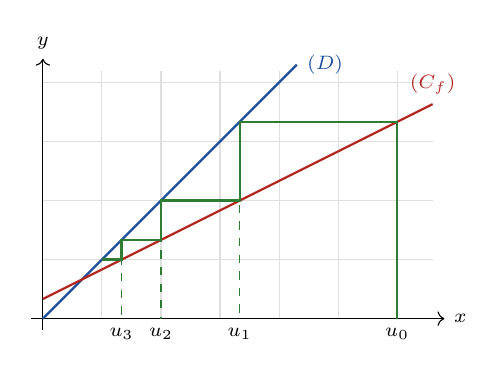
\begin{tikzpicture}[scale=0.75,font=\scriptsize]
\draw[gray!25] (0,0) grid (6.6,4.2);
\draw[->] (-0.2,0)--(6.8,0) node[right]{$x$}; \draw[->] (0,-0.2)--(0,4.4) node[above]{$y$};
\draw[cDef,thick] (0,0)--(4.3,4.3) node[right]{$(D)$};
\draw[cThm,thick] (0,0.333)--(6.6,3.633) node[above]{$(C_f)$};
\draw[cRem,thick] (6,0)--(6,3.333)--(3.333,3.333)--(3.333,2)--(2,2)--(2,1.333)--(1.333,1.333)--(1.333,1)--(1,1);
\draw[cRem,dashed] (3.333,3.333)--(3.333,0) (2,2)--(2,0) (1.333,1.333)--(1.333,0);
\foreach \x/\n in {6/u_0,3.333/u_1,2/u_2,1.333/u_3} \node[below] at (\x,0){$\n$};
\end{tikzpicture}
\end{LTR}}
\end{mithal}

% =====================================================================
\section{اتجاه تغير متتالية}
\begin{tarif}
لتكن $\Un_{n\ge n_0}$ متتالية عددية. نقول إن $\Un$:
\begin{itemize}
\item \textbf{متزايدة تماماً} إذا كان من أجل كل $n\ge n_0$: \ $u_{n+1}>u_n$.
\item \textbf{متناقصة تماماً} إذا كان من أجل كل $n\ge n_0$: \ $u_{n+1}<u_n$.
\item \textbf{ثابتة} إذا كان من أجل كل $n\ge n_0$: \ $u_{n+1}=u_n$.
\end{itemize}
\end{tarif}
\begin{tariqa}[ثلاث طرق لدراسة اتجاه التغير]
\begin{enumerate}
\item \textbf{إشارة الفرق} $u_{n+1}-u_n$: \ إذا كان موجباً تماماً فإن $\Un$ متزايدة تماماً ، وإذا كان سالباً تماماً فهي متناقصة تماماً.
\item \textbf{مقارنة النسبة} $\dfrac{u_{n+1}}{u_n}$ \textbf{بالعدد $1$} \ (فقط إذا كانت كل الحدود \textbf{موجبة تماماً}): \ $\dfrac{u_{n+1}}{u_n}>1$ معناه متزايدة تماماً ، و $\dfrac{u_{n+1}}{u_n}<1$ معناه متناقصة تماماً.
\item \textbf{الدالة المرفقة} (إذا كان $u_n=f(n)$): إذا كانت $f$ متزايدة (متناقصة) على $[n_0;+\infty[$ فإن $\Un$ متزايدة (متناقصة).
\end{enumerate}
\end{tariqa}
\begin{mithal}
\begin{itemize}
\item $u_n=n^2+n$: \ $u_{n+1}-u_n=(n+1)^2+(n+1)-n^2-n=2n+2>0$ ، إذن $\Un$ \textbf{متزايدة تماماً}.
\item $v_n=\dfrac{3^n}{n+4}>0$: \ $\dfrac{v_{n+1}}{v_n}=\dfrac{3^{n+1}}{n+5}\times\dfrac{n+4}{3^n}=\dfrac{3(n+4)}{n+5}$ ، و $\dfrac{3(n+4)}{n+5}-1=\dfrac{2n+7}{n+5}>0$: \ $(v_n)$ \textbf{متزايدة تماماً}.
\item $w_n=-2n+3=f(n)$ حيث $f(x)=-2x+3$ متناقصة تماماً على $[0;+\infty[$: \ $(w_n)$ \textbf{متناقصة تماماً}.
\end{itemize}
\end{mithal}
\begin{molahada}
عكس الطريقة 3 خاطئ: إذا كانت $u_{n+1}=f(u_n)$ و $f$ متزايدة ، فلا نستنتج أن $\Un$ متزايدة. \ (مع $f(x)=\dfrac12x+\dfrac13$ المتزايدة ، المتتالية السابقة متناقصة.)
\end{molahada}

% =====================================================================
\section{المتتاليات المحدودة}
\begin{tarif}[متتالية محدودة]
$\Un$ \textbf{محدودة من الأعلى} إذا وجد عدد $M$ حيث $u_n\le M$ لكل $n$ ، و\textbf{محدودة من الأسفل} إذا وجد $m$ حيث $u_n\ge m$ لكل $n$. \ وهي \textbf{محدودة} إذا كانت محدودة من الأعلى ومن الأسفل.
\end{tarif}
\begin{mithal}
$u_n=2+\dfrac{1}{n+1}$ ، $n\in\N$. \ من أجل كل $n\in\N$: \ $n+1\ge1$ ، إذن $0<\dfrac{1}{n+1}\le1$ ، ومنه \bx{2<u_n\le3}.\par
$\Un$ محدودة من الأسفل بـ $2$ ومن الأعلى بـ $3$ ، فهي \textbf{محدودة}.
\end{mithal}
\begin{tariqa}[إثبات أن متتالية محدودة]
نكتب $u_n$ بدلالة $n$ (الحد العام) ثم ننطلق من $n\ge n_0$ ونطبّق العمليات على المتباينات ، أو ندرس إشارة الفرق $u_n-a$.
\end{tariqa}

% =====================================================================
\section{المتتاليات الحسابية}
\begin{tarif}
نقول إن $\Un$ \textbf{متتالية حسابية} إذا وجد عدد حقيقي $r$ حيث من أجل كل $n$: \ \bx{u_{n+1}=u_n+r}.\par
العدد $r$ يسمى \textbf{أساس} المتتالية (ننتقل من حد إلى الذي يليه بإضافة نفس العدد $r$).
\end{tarif}
\begin{tariqa}[إثبات أن متتالية حسابية]
نحسب $u_{n+1}-u_n$ ، فإذا وجدناه \textbf{عدداً ثابتاً} $r$ (لا يتعلق بـ $n$) فإن $\Un$ حسابية أساسها $r$.
\end{tariqa}
\begin{khassia}[الحد العام]
\begin{itemize}
\item إذا كان الحد الأول $u_0$: \ \bx{u_n=u_0+nr} \quad ؛ \quad إذا كان الحد الأول $u_1$: \ \bx{u_n=u_1+(n-1)r}.
\item بصفة عامة ، من أجل كل عددين طبيعيين $n$ و $p$: \ \bx{u_n=u_p+(n-p)r}.
\end{itemize}
\end{khassia}
\begin{khassia}[اتجاه التغير]
\begin{itemize}
\item إذا كان $r>0$ فإن $\Un$ متزايدة تماماً. \quad إذا كان $r<0$ فإن $\Un$ متناقصة تماماً. \quad إذا كان $r=0$ فإن $\Un$ ثابتة.
\end{itemize}
\end{khassia}
\begin{khassia}[ثلاثة حدود متتابعة]
الأعداد $a$ ، $b$ ، $c$ بهذا الترتيب حدود متتابعة من متتالية حسابية إذا وفقط إذا كان \bx{a+c=2b}. \ ($b$ هو \textbf{الوسط الحسابي} لـ $a$ و $c$.) \ مثال: $2$ ، $7$ ، $12$ لأن $2+12=2\times7$.
\end{khassia}
\begin{khassia}[مجموع حدود متتابعة]
\[\bx{S=\text{\ar{عدد الحدود}}\times\frac{\text{\ar{الحد الأول}}+\text{\ar{الحد الأخير}}}{2}}\qquad;\qquad u_0+u_1+\cdots+u_n=(n+1)\,\frac{u_0+u_n}{2}.\]
عدد الحدود $=$ (دليل الحد الأخير $-$ دليل الحد الأول) $+1$. \ حالة خاصة: $1+2+\cdots+n=\dfrac{n(n+1)}{2}$.
\end{khassia}
\begin{mithal}
\begin{itemize}
\item $u_n=3n+5$: \ $u_{n+1}-u_n=3$ ، فهي حسابية أساسها $r=3$ وحدها الأول $u_0=5$.
\item $\Un$ حسابية ، $u_0=7$ و $u_{32}=103$: \ $r=\dfrac{103-7}{32}=3$ ، و $u_0+\cdots+u_{32}=33\times\dfrac{7+103}{2}=\bx{1815}$.
\end{itemize}
\end{mithal}

% =====================================================================
\section{المتتاليات الهندسية}
\begin{tarif}
نقول إن $\Un$ \textbf{متتالية هندسية} إذا وجد عدد حقيقي $q$ حيث من أجل كل $n$: \ \bx{u_{n+1}=q\times u_n}.\par
العدد $q$ يسمى \textbf{أساس} المتتالية (ننتقل من حد إلى الذي يليه بالضرب في نفس العدد $q$).
\end{tarif}
\begin{tariqa}[إثبات أن متتالية هندسية]
نعبّر عن $v_{n+1}$ بدلالة $v_n$ ونصل إلى الشكل $v_{n+1}=q\,v_n$ ، أو (إذا كانت الحدود غير معدومة) نبيّن أن $\dfrac{v_{n+1}}{v_n}$ ثابت.
\end{tariqa}
\begin{khassia}[الحد العام]
\begin{itemize}
\item إذا كان الحد الأول $u_0$: \ \bx{u_n=u_0\times q^n} \quad ؛ \quad إذا كان الحد الأول $u_1$: \ \bx{u_n=u_1\times q^{n-1}}.
\item بصفة عامة: \ \bx{u_n=u_p\times q^{n-p}}.
\end{itemize}
\end{khassia}
\begin{khassia}[اتجاه التغير (حالة $u_0>0$)]
\begin{itemize}
\item إذا كان $q>1$: $\Un$ متزايدة تماماً. \quad إذا كان $0<q<1$: متناقصة تماماً. \quad إذا كان $q=1$: ثابتة.
\item إذا كان $u_0<0$ ينعكس الاتجاه ، وإذا كان $q<0$ فالمتتالية \textbf{ليست رتيبة} (الإشارات تتناوب).
\end{itemize}
\end{khassia}
\begin{khassia}[ثلاثة حدود متتابعة]
الأعداد $a$ ، $b$ ، $c$ بهذا الترتيب حدود متتابعة من متتالية هندسية إذا وفقط إذا كان \bx{a\times c=b^2}. \ ($b$ هو \textbf{الوسط الهندسي}.) \ مثال: $1$ ، $5$ ، $25$ لأن $1\times25=5^2$.
\end{khassia}
\begin{khassia}[مجموع حدود متتابعة ($q\ne1$)]
\[\bx{S=\text{\ar{الحد الأول}}\times\frac{1-q^{\,\text{\ar{عدد الحدود}}}}{1-q}}\qquad;\qquad u_0+u_1+\cdots+u_n=u_0\,\frac{1-q^{n+1}}{1-q}.\]
إذا كان $q=1$: \ $u_0+\cdots+u_n=(n+1)u_0$.
\end{khassia}
\begin{mithal}
\begin{itemize}
\item $v_n=\dfrac{3}{2^n}$: \ $v_{n+1}=\dfrac{3}{2^{n}\times2}=\dfrac12v_n$ ، فهي هندسية أساسها $q=\dfrac12$ وحدها الأول $v_0=3$.
\item $u_0=2$ و $q=3$: \ $u_0+\cdots+u_n=2\times\dfrac{1-3^{n+1}}{1-3}=\bx{3^{n+1}-1}$.
\end{itemize}
\end{mithal}

% =====================================================================
\section{نهاية متتالية وخلاصة الطرائق}
\begin{tarif}
\begin{itemize}
\item نقول إن $\Un$ \textbf{متقاربة} نحو العدد الحقيقي $\ell$ إذا كان كل مجال مفتوح يشمل $\ell$ يشمل كل حدود المتتالية ابتداءً من رتبة معيّنة ، ونكتب $\limn u_n=\ell$. \ النهاية إن وجدت فهي وحيدة.
\item المتتالية غير المتقاربة تسمى \textbf{متباعدة}: نهايتها $+\infty$ أو $-\infty$ أو غير موجودة.
\end{itemize}
\end{tarif}
\begin{khassia}[متتالية من الشكل $u_n=f(n)$]
إذا كانت $\displaystyle\lim_{x\to+\infty}f(x)=\ell$ (أو $\pm\infty$) فإن $\limn u_n=\ell$ (أو $\pm\infty$). \ كل نظريات نهايات الدوال تبقى صحيحة.
\end{khassia}
\begin{mithal}
$v_n=\dfrac{2n+1}{n+3}$: \ $\limn v_n=\displaystyle\lim_{x\to+\infty}\frac{2x}{x}=\bx{2}$. \quad $u_n=-n^2$: \ $\limn u_n=-\infty$. \quad $u_n=2+(-1)^n$: لا تقبل نهاية (تتناوب بين $1$ و $3$).
\end{mithal}
\begin{khassia}[نهاية متتالية هندسية $u_n=u_0\,q^n$ ($u_0\ne0$)]
\renewcommand{\arraystretch}{1.5}
\centering
\begin{tabular}{|c|c|c|c|c|}\hline
\cellcolor{cThm!15}$q$ & $q\le-1$ & $-1<q<1$ & $q=1$ & $q>1$\\\hline
\cellcolor{cThm!15}$\limn q^n$ & غير موجودة & $0$ & $1$ & $+\infty$\\\hline
\cellcolor{cThm!15}$\limn u_n$ & غير موجودة & $0$ & $u_0$ & $+\infty$ إذا $u_0>0$ ، $-\infty$ إذا $u_0<0$\\\hline
\end{tabular}
\end{khassia}
\begin{mithal}
$u_n=\Big(\dfrac{-3}{4}\Big)^n$: \ $-1<-\dfrac34<1$ ، إذن $\limn u_n=0$. \quad $v_n=-2\times6^n$: \ $q=6>1$ و $v_0=-2<0$ ، إذن $\limn v_n=-\infty$.
\end{mithal}
\begin{tmr}
$u_0=2$ و $u_{n+1}=1+\dfrac25u_n$. \ نضع $v_n=u_n-\dfrac53$.
\begin{enumerate}
\item بيّن أن $(v_n)$ هندسية يطلب تعيين أساسها وحدها الأول.
\item اكتب $u_n$ بدلالة $n$ ، ثم عيّن $\limn u_n$.
\end{enumerate}
\end{tmr}
\begin{hal}
\textbf{1.} $v_{n+1}=u_{n+1}-\dfrac53=1+\dfrac25u_n-\dfrac53=\dfrac25u_n-\dfrac23=\dfrac25\Big(u_n-\dfrac53\Big)=\dfrac25v_n$.\par
$(v_n)$ هندسية أساسها \bx{q=\dfrac25} وحدها الأول $v_0=2-\dfrac53=\bx{\dfrac13}$.
\QQ{2} $v_n=\dfrac13\Big(\dfrac25\Big)^n$ ، و $u_n=v_n+\dfrac53=\bx{\dfrac53+\dfrac13\Big(\dfrac25\Big)^n}$. \ بما أن $0<\dfrac25<1$: $\limn\Big(\dfrac25\Big)^n=0$ ، إذن $\limn u_n=\bx{\dfrac53}$.
\end{hal}
\begin{BOX}{cMeth}{مقارنة بين المتتاليتين الحسابية والهندسية}
\renewcommand{\arraystretch}{1.6}
\centering
\begin{tabular}{|M{0.3\textwidth}|M{0.3\textwidth}|M{0.24\textwidth}|}\hline
\cellcolor{cMeth!15}\textbf{هندسية أساسها $q$} & \cellcolor{cMeth!15}\textbf{حسابية أساسها $r$} & \cellcolor{cMeth!15}\textbf{الخاصية}\\\hline
$u_{n+1}=q\,u_n$ & $u_{n+1}=u_n+r$ & التعريف\\\hline
$u_n=u_0\,q^n=u_p\,q^{n-p}$ & $u_n=u_0+nr=u_p+(n-p)r$ & الحد العام\\\hline
$a\times c=b^2$ & $a+c=2b$ & ثلاثة حدود متتابعة\\\hline
$u_0\dfrac{1-q^{n+1}}{1-q}$ \ ($q\ne1$) & $(n+1)\dfrac{u_0+u_n}{2}$ & $u_0+u_1+\cdots+u_n$\\\hline
\end{tabular}
\end{BOX}
\begin{BOX}{cMeth}{ماذا أفعل عندما يُطلب مني $\ldots$؟}
\renewcommand{\arraystretch}{1.5}
\centering
\begin{tabular}{|p{0.56\textwidth}|p{0.32\textwidth}|}\hline
\cellcolor{cMeth!15}\textbf{الطريقة} & \cellcolor{cMeth!15}\textbf{المطلوب}\\\hline
إشارة $u_{n+1}-u_n$ ، أو مقارنة $\dfrac{u_{n+1}}{u_n}$ بـ $1$ ، أو الدالة المرفقة. & اتجاه التغير\\\hline
نبيّن أن $u_{n+1}-u_n=r$ ثابت. & إثبات أن $\Un$ حسابية\\\hline
نكتب $v_{n+1}$ بدلالة $u_n$ ثم نُخرج $q$ عاملاً: $v_{n+1}=q\,v_n$. & إثبات أن $(v_n)$ هندسية\\\hline
نكتب $v_n$ بدلالة $n$ ، ثم نعوّض في العلاقة بين $u_n$ و $v_n$. & $u_n$ بدلالة $n$\\\hline
نحل المعادلة $u_n=a$ في $\N$ ؛ الرتبة $=n-n_0+1$. & هل $a$ حد من حدودها؟\\\hline
نكتب $u_n$ بدلالة $n$ ثم ننطلق من $n\ge n_0$ ، أو ندرس إشارة $u_n-a$. & حصر الحدود $u_n>a$\\\hline
$S'=u_0+\cdots+u_n$: نكتب $u_k=v_k+c$ فنجد $S'=S+(n+1)c$. & مجموع $u_k$ إذا $u_k=v_k+c$\\\hline
\end{tabular}
\end{BOX}

\end{document}
